% !TEX root = ../main.tex
% Chapter 1

\chapter{Introduction}

\label{Chapter1} % For referencing the chapter elsewhere, use~\ref{Chapter1}

\lhead{Chapter 1. \emph{Introduction}} % This is for the header on each page - perhaps a shortened title

%----------------------------------------------------------------------------------------

\section{Outline}
\emph{Not intented for the reader.}
\begin{itemize}
  \item Context of research (\gls{har}), real-world applications
  \item Current methods, wrapper vs. filter methods
  \item Problem statement with current filter methods (which follows from Chapter~\ref{Chapter3} which goes in-depth with methods).
  \item Purpose of this research. E.g. "Find a better algorithm for short-activity segmentation"
  \item Provide the \emph{motivation} for this approach
  \item Relate to real-world applications
  \item Outline for rest of the thesis
\end{itemize}

-- Overall todo's --
\begin{itemize}
  \item \TODO{The term \emph{emperical data/distruction} is nowhere used in the thesis. or: Emperical cumulative distribution. Especially Chapter 2.}
  \item \TODO{Check for ``tang-constructions'': saying to much in a single sentence.}
  \item \TODO{Overall: meer focus op de \emph{waarom} vraag/antwoord bij keuzes. Bouwt aan motivatie en context van het geheel.}
  \item \TODO{Nu staat nog veel (met name Chapter 2) in ``aantekening'' style; ombouwen naar uitleggen, lezer begeleiden, duiden, verlaren etc.}
  \item \TODO{Test moet condenser: bepalen wat er uit gelaten mag worden.}
\end{itemize}

\begin{figure}
  \centering
    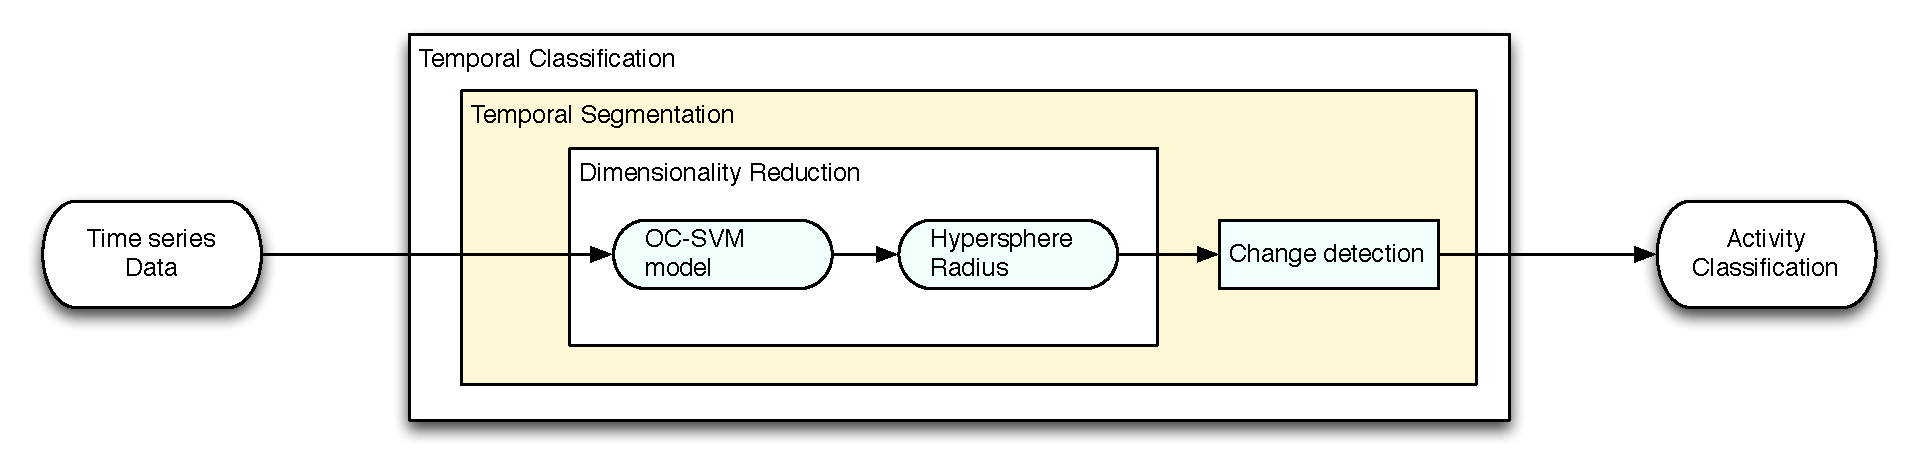
\includegraphics[width=\textwidth,height=\textheight,keepaspectratio]{./Figures/chapter1/thesis_goal.pdf}
  \caption[Thesis goal]{The goal of this thesis. The scope of this thesis is Temporal Segmentation, which can be useful in the context of Temporal Classification. Given a data set, we apply the construction of \gls{oc-svm} models as a form of dimensionality reduction. Using the reduced representation, being the radius $R$ of the constructed hypersphere, we apply direct change detection methods. The detected change points can support the classification of homogeneous segments of data.}
  \label{fig:thesis_goal}
\end{figure}